\chapter{Informatie}

\section{Opdacht 1}
\emph{Een roulettespel heeft een draaischijf met 38 genummerde vakjes: 18 rode, 18 zwarte en 2 groene vakjes. Op de draaiende schijf wordt een balletje geworpen. Als de schijf tot rust komt, zal het balletje in \'{e}\'{e}n van de vakjes blijven liggen. Elk vakje heeft evenveel kans om het balletje te vangen. De zwarte vakjes zijn oneven genummerd van 1, 3, 5, \ldots, 35, de rode vakjes zijn even genummerd van 2, 4, 6, \ldots, 36 en de twee groene vakjes hebben de 'nummers' 0 en 00. Zodra de croupier de kleur of het nummer van het winnende vakje genoemd heeft, mag er niet meer ingezet worden.}
\begin{itemize}
  \item[(a)] \emph{Hoe groot is de selectieve informatie over elke kleur van het vakje? \emph{1 bit}}\\
    $ld(1/p)$ waar $p$ de kans op een kleur is.\\\\
    \begin{tabular}{|l|l||l|}\hline
      Rood & $ld(38/18)$ & 1,078 bits \\\hline
      Zwart & $ld(38/18)$ & 1,078 bits \\\hline
      Groen & $ld(38/2)$ & 4,248 bits \\\hline
    \end{tabular}

  \item[(b)] \emph{Hoe groot is de gemiddelde informatie over de kleur van het vakje? \emph{1 bit}}\\
    Het complement van de som $p_i \cdot ld(p_i)$ voor iedere $i$\\
    
    $(18/38) \cdot ld(18/38) + (18/38) \cdot ld(18/38) + (2/38) \cdot ld(2/38)) = 1.245 bits$
    
  \item[(c)] \emph{Hoe groot is de gemiddelde informatie over het nummer van het vakje? \emph{$(2*6+16*5+8*4+4*3+2*2+1*1)/38=3.71bit$}}\\
    
    Het complement van de som $p_i \cdot ld(p_i)$ voor idere $i$.\\
    
    Er zijn 38 mogelijke getallen, met iedere een gelijke kans:
    $(-(1/38) \cdot ld(1/38))*38 = ld(38) = 5.248 bits$

  \item[(d)] \emph{Hoe groot is de conditionele entropie (equivocatie) van de kleur als het nummer van het vakje al bekend is?}\\
    
  Als je het nummer weet, weet je ook de kleur. in andere woorden: De kleur is volledig afhankelijk van het getal. Conditionele entropie is daarom $0$
    
   \item[(e)] \emph{Hoe groot is de conditionele entropie (equivocatie) van het nummer als de kleur van het vakje al bebend is? }}\\
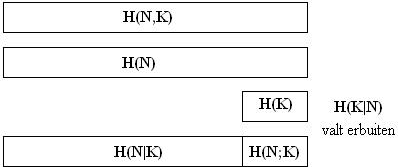
\includegraphics{h1.png}
\end{itemize}


\section{Opdracht 4}
\emph{Volgens bijlage D komen in normale teksten korte woorden frequenter voor dan lange woorden. In het 'Groene boekje' woordenlijst van de Nederlandse taal) blijkt dat niet te kloppen.  Geef hier een verklaring voor.}

De drie bestaande lidwoorden zijn veel gebruikte woorden in de Nederlandse taal. Lidwoorden worden vaker gebruikt als ``normale'' woorden, waardoor de verhouding hierdoor al niet klopt. Maar bijvoorbeeld ook werkwoorden en ook persoonsvormen zijn gemiddeld genomen korter. Er zijn dus wel meer verschillende lange woorden, maar die worden minder ``hergebruikt'' als de eerder genoemde korte woorden. 

\section{Opdracht 5}
\emph{Binare Coded Decimals ('BCD') is een code waarbij een getal van 0, 1, 2, \ldots, 99 in een 8 bit-woord (een '\emph{byte}') gecodeerd wort. Hoeveel redundantie bevat zo'n BCD-woord?}

100 mogelijke BCD waarde, $H(X)=ld(100)=6.64$
256 combinaties met een byte, ofwel 8 bits.

$8-6.64=1.36$ bits
